\section{Introduction}

\begin{wrapfigure}[18]{r}{0.45\textwidth}
   \vspace{-40pt}
   \centering
   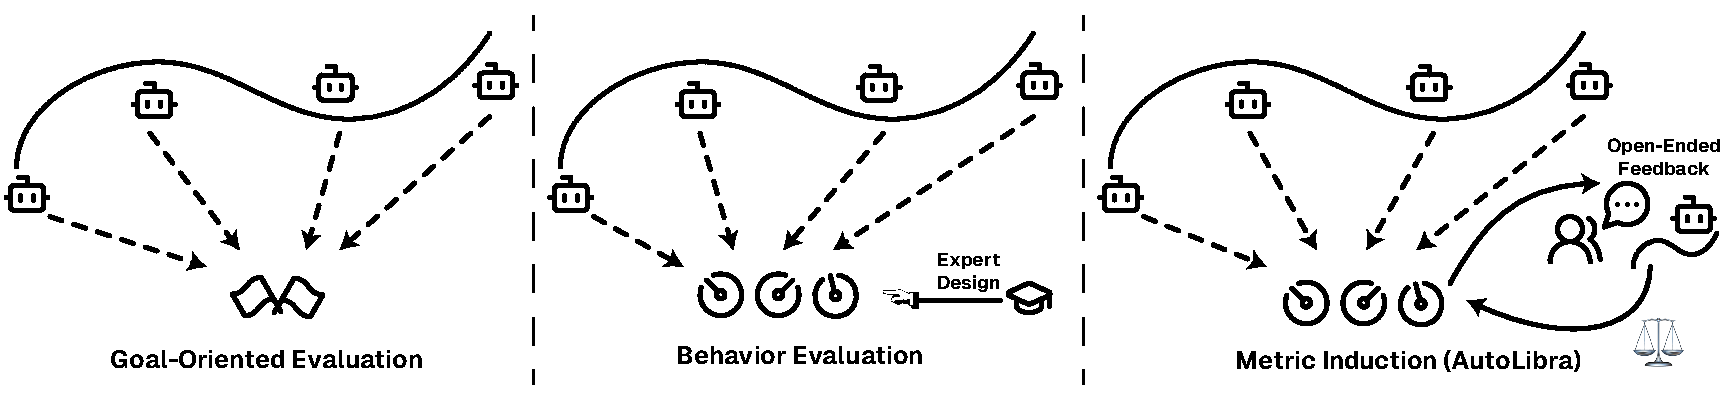
\includegraphics[width=0.45\textwidth]{figs/autolibra.pdf}
   \caption{AutoLibra provides behavioral evaluation on agent performance
    through automatic metric induction based on human feedback and agent trajectories.}
\end{wrapfigure}


Efficient human learners internalize open-ended feedback from others into self-regulation metrics
\citep{pintrich2002development,nicol2006formative}.
These metrics offer lenses for self-reflection on the
strengths and weaknesses of ourselves and ladders for self-improvement.
In this paper, we ask:
\textbf{can we automatically induce metrics to evaluate and improve language agents from natural language feedback?} 

   
The current evaluation of large language model (LLM) agents and reward modeling often fall
into two paradigms: (1) goal-oriented evaluation --
\emph{whether the agents have fulfilled the given task},
\emph{e.g.} benchmarks \citep{zhouwebarena,jimenezswe,chan2024mle,paglieri2024balrog} and reward
modeling approaches \citep{pan2024autonomous,chen2025scaling,choudhury2025process}
and (2) behavior evaluation -- \emph{how well the agents do on heuristically designed dimensions},
\emph{e.g.} social agent and human-agent interaction benchmarks \citep{zhousotopia,shao2024collaborative}
and agent failure mode analysis \citep{pan2025why,zhang2023effects,yang2023behavioral}. 
Goal-oriented evaluation is often designed to be verifiable through considering, but it is not fine-grained
or comprehensive enough to diagnose agents' behavior problems or find the bottlenecks for improvements \citep{yehudai2025survey}.  
While behavior evaluation complements it, it requires manual design of the metrics either based on top-down heuristics
\citep{zhousotopia}, or thematic analysis of the agent's behavior \citep{shao2024collaborative,pan2025why}.
This manual design process is often time-consuming and labor-intensive through expert annotations and classifications. 

We introduce AutoLibra \protect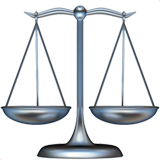
\includegraphics[height=1em]{figs/scale.png}, an automatic metric induction method,
as a new paradigm for agent evaluation and improvement.
This method offers behavior evaluation for agents, while (1) automating the metric creation process with LLMs, 
(2) optimizing the alignment through searching for a set of metrics to cover human feedback with minimal redundancy,
and (3) providing concrete examples of good and bad behaviors for each metric to improve the
LLM-as-a-Judge's performance. 
\begin{wrapfigure}{r}{0.7\textwidth}
    \centering
    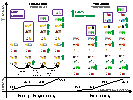
\includegraphics[width=0.7\textwidth]{figs/autolibra-teaser.pdf}
    \caption{Caption}
    \label{fig:enter-label}
\end{wrapfigure}

AutoLibra takes in agent trajectories along with human open-ended feedback, and generates a set of metrics, each with a name, description, and a list of good behavior examples, and bad behavior examples. AutoLibra 



